\section{Solution}

% Solution: describes your solution of the task.
% Contains a detailed description of all the subtasks which have been solved and how they contribute to the solution for the given task.
% The use of diagrams, figures, tables and similar is welcome as a support to your description.

% TODO: Putt dette i introduksjonen? Eventuelt putt lista i et vedlegg
\subsection{Tools}

Development was done on computers in the computer lab running Ubuntu 12.04.
In addition, we used Microsoft Remote Desktop to be able to use Xilinx from other locations.
ghdl and gtkwave also proved useful, as it allowed us to work locally when only writing and testing vhdl modules. Figure \ref{fig:software} lists all the software used.

\begin{figure}[ht!]
    \begin{description}
        \item{\textbf{ISE Project Navigator 12.4 M.81d}}
            Main IDE for writing and synthesizing VHDL.
        \item{\textbf{ISim 12.4 M.81d}}
            Simulation environment for simulating VHDL.
        \item{\textbf{hostcomm 1.0.0}}
            Programming utility for the Spartan-6 LX16 Evaluation Kit.
        \item{\textbf{VIM}}
            For text editing.
        \item{\textbf{GHDL}}
            Allowed for writing and testing components on Mac OS X.
        \item{\textbf{gtkwave}}
            Visualization tool for inspecting test simulations run with ghdl.
        \item{\textbf{git \& GitHub}}
            Version control system with central code repository hosting.
    \label{fig:software}
    \end{description}
    \caption{Software used during the development process}
\end{figure}

\subsection{Architecture}

The suggested architecture for the project provided in Figure 4.1 [1, p.45] was abandoned in favor of a design based on the basic multi cycle architecture presented in lecture 4 [2].

As the host environment was tailored towards the single cycle MIPS architecture, notably including separate instruction and data memory (harvard architecture) as well as byte addressable memory, the architecture received slight modifications.

There's no dedicated component for executing memory reads and writes.
Instead, components responsible for computing memory addresses interface with memory directly, and incoming memory data buses are connected directly to instruction- and other registers.
As the external memory has one cycle response delay, some of the suggested datapath registers were removed.

Additional extensions to the architecture include support for the load upper immediate instruction, as well ass SLL and SRL functions.
The RTL sketch of the final design can be seen in figure \ref{fig:top_level_rtl}.

\subsubsection{MIPS subset}

The final processor design implements the following subset of the MIPS instruction set.

\begin{itemize}
    \item ALU instructions (ADD, SUB, SLT, AND, OR, SLL, SRL)
    \item Conditional Branch (BEZ)
    \item Jump Instruction (JMP)
    \item LOAD, STORE, Load immediate (LW, SW, LDI)
\end{itemize}

Note: the {\bf LDI} (Load Immediate) instruction is not a part of the MIPS instruction set\footnote{Figure C.1 \cite[p.66]{compendium}}.
The {\bf LUI} (Load Upper Immediate) is the closest match.
This instruction loads the value into the upper 16 bits of the register.
The support files handed out already use this instruction.

\subsubsection{Control unit}

The control unit is based on the state machine from lecture 4 \cite{lecture-4}.
It has been modified to add support for the extra load upper immediate instruction.
Output signals which were not needed in our architecture are also removed.
Specifically, the i\_or\_d and mem\_read signals were not needed, as our processor has separate instruction and data memories.

Because of the one cycle latency when reading from external memory, the ir\_write signal has been moved to the instruction\_decode state, when the correct instruction has been fetched.
This does not cause any latency issues, as the instruction register is designed to let the new instruction value pass through when ir\_write is high.
A state diagram for the control unit can be seen in figure \ref{fig:state_machine}.

The control unit takes two inputs, the current opcode (first 6 bits of the instruction) and a processor enable signal.
When the processor is disabled, the state machine should stay in the idle state.

The outputs from the state machine are dependent only on the current state.
This makes it a Moore machine.

\begin{figure}[ht!]
    \begin{center}
    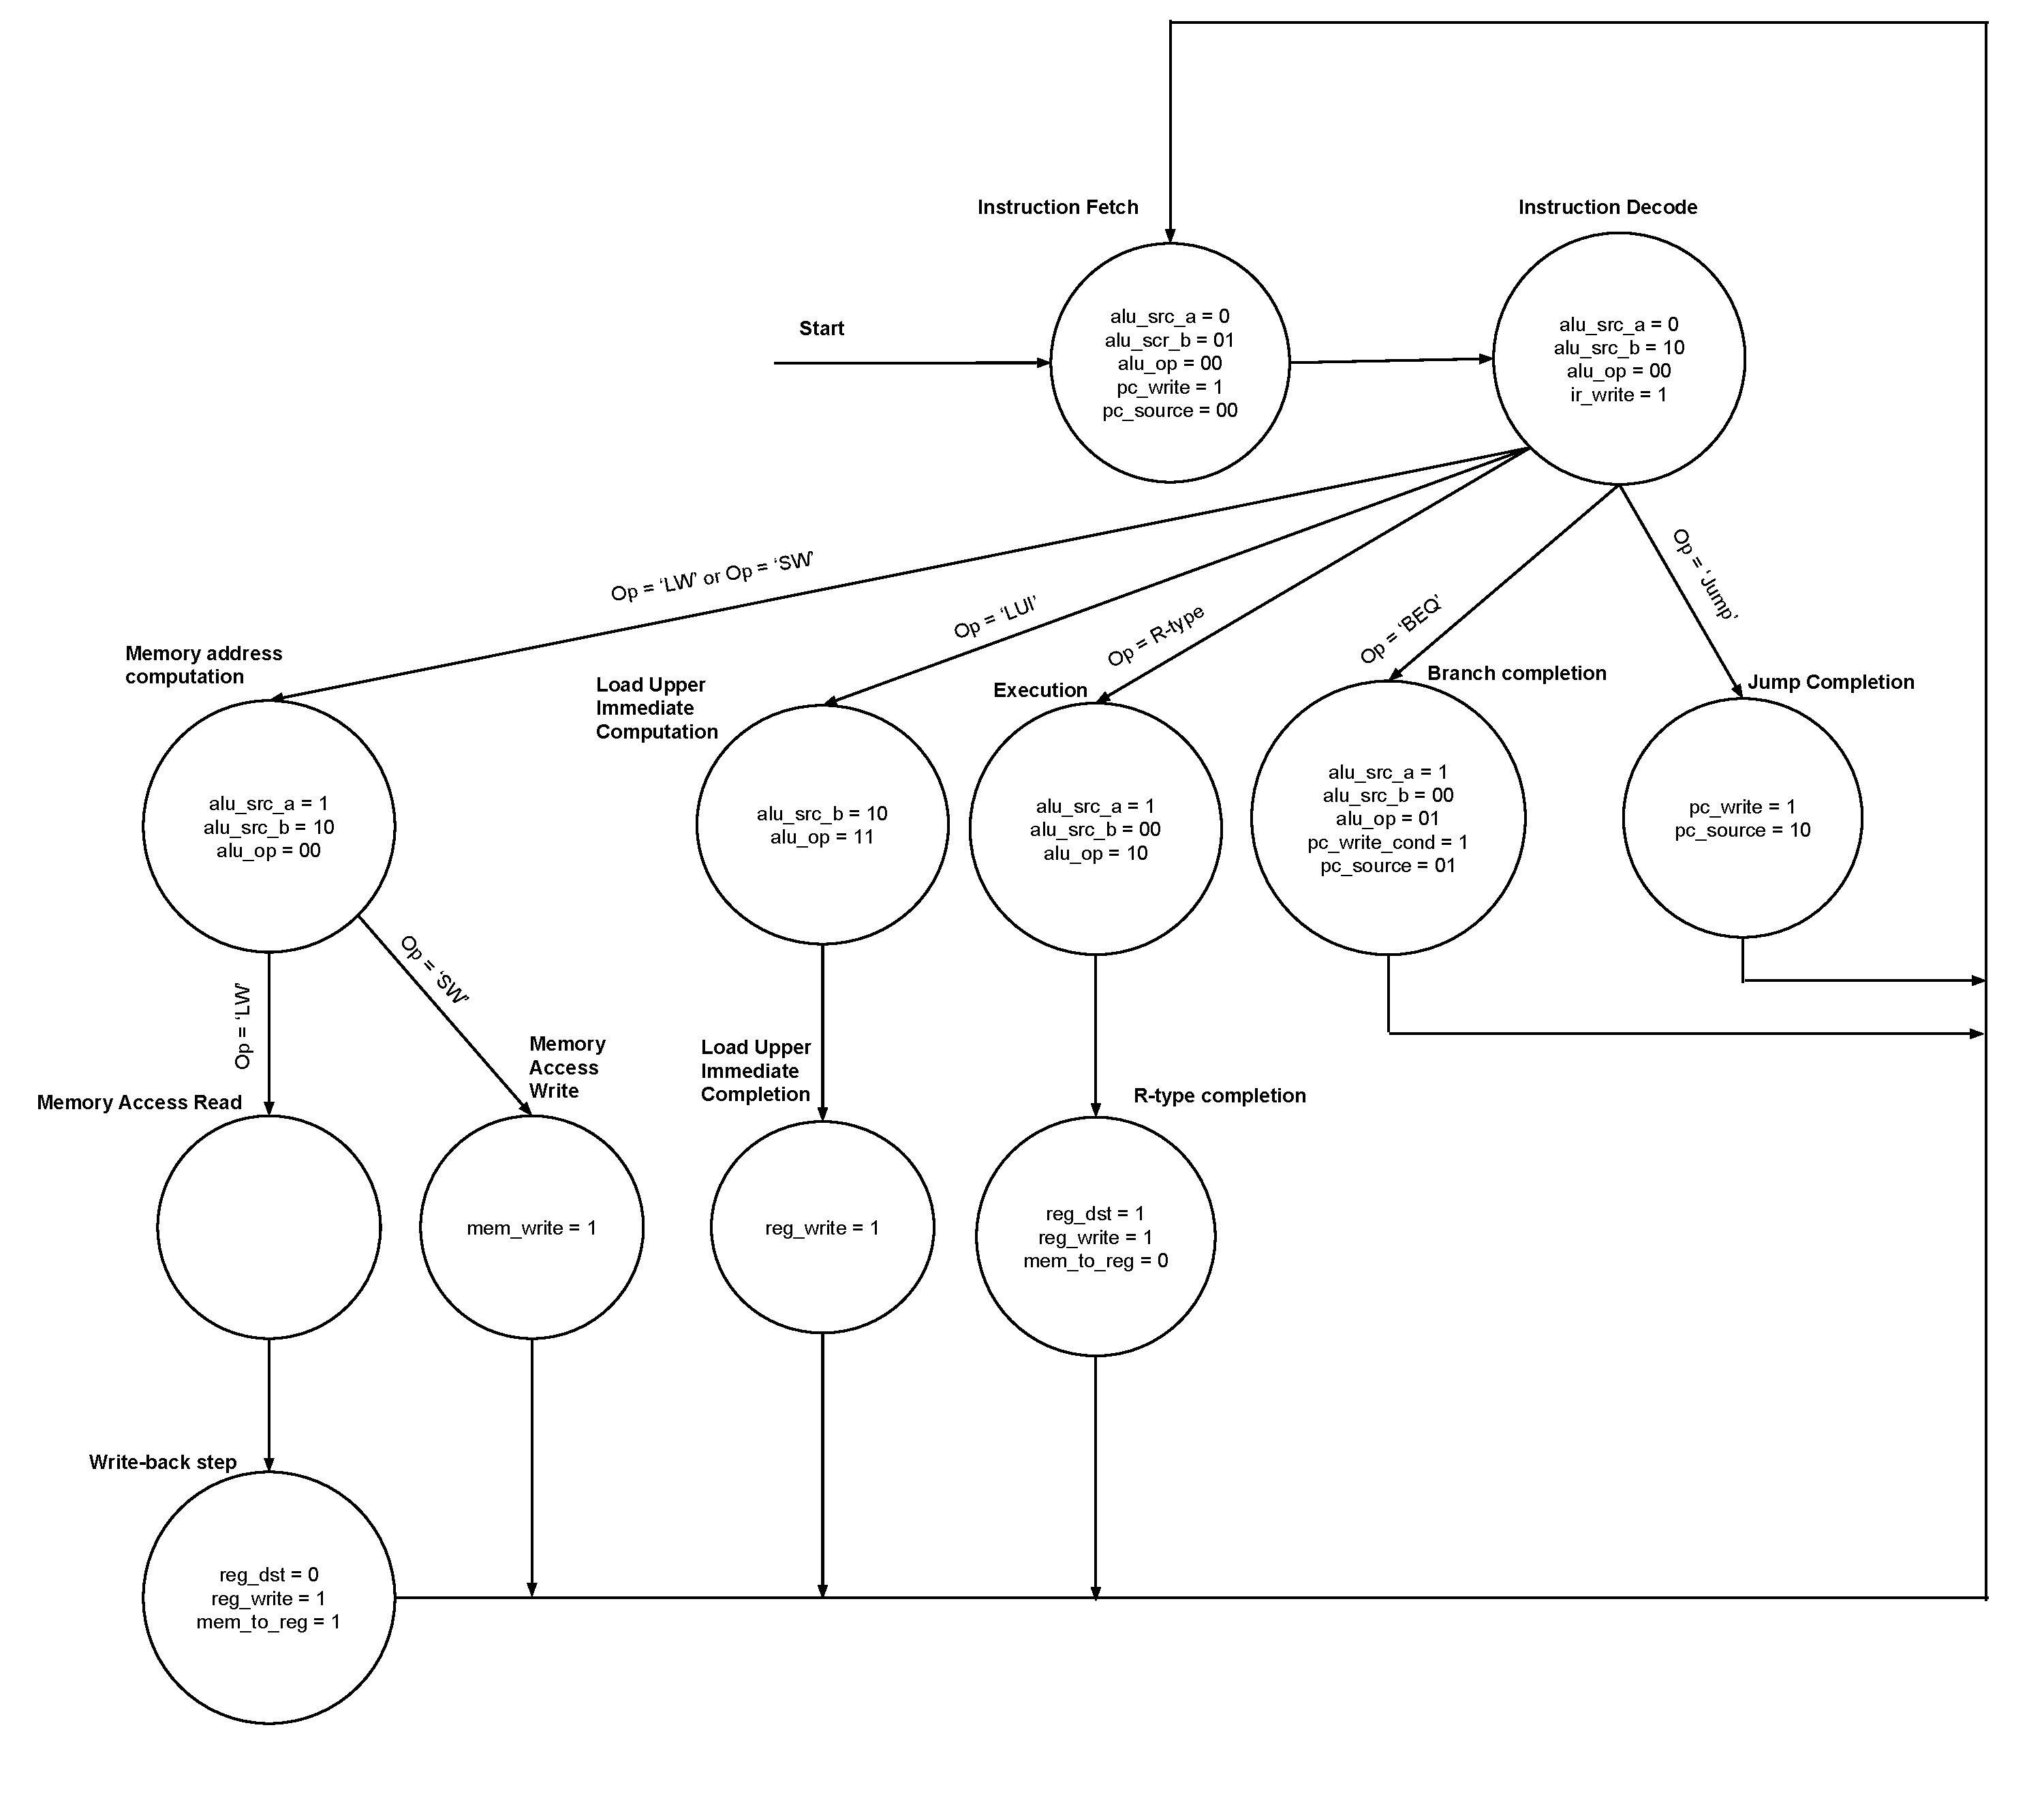
\includegraphics[width=\textwidth]{assets/state_machine.pdf}
    \caption{State diagram for the control unit}
    \label{fig:state_machine}
    \end{center}
\end{figure}

\subsection{Implementation}

A modular approach was taken when implementing the system.
An interface was defined for each component, defining which inputs and outputs it should have,
and describing how it should perform.
Their functionality were verified with separate testbenches, which meant that they could be developed independently of each other.
This way, we were able to develop components in parallel.
Different components are detailed below.

\subsubsection{Instruction register}

Caches instructions while their executed.

\subsubsection{Register file}

Stores data.

\subsubsection{ALU Control}

\begin{table}[ht!]
    \begin{tabular}{|l|l|l|l|l|l|l|}
    \hline
    Opcode & ALUOp & Operation           & Function & ALU Control & Shamt   \\ \hline
    lw     & 00    & load word           & XXXXXX   & ADD         & XXXXX \\ \hline
    sw     & 00    & store word          & XXXXXX   & ADD         & XXXXX \\ \hline
    beq    & 01    & branch equal        & XXXXXX   & SUBTRACT    & XXXXX \\ \hline
    r-type & 10    & add                 & 100000   & ADD         & XXXXX \\ \cline{3-6}
           &       & subtract            & 100010   & SUBTRACT    & XXXXX \\ \cline{3-6}
           &       & AND                 & 100100   & AND         & XXXXX \\ \cline{3-6}
           &       & OR                  & 100101   & OR          & XXXXX \\ \cline{3-6}
           &       & set-on-less-than    & 101010   & SLT         & XXXXX \\ \cline{3-6}
           &       & shift-left-logical  & 000000   & SLL         & Pass through \\ \cline{3-6}
           &       & shift-right-logical & 000010   & SRL         & Pass through \\ \hline
    lui    & 11    & lui                 & XXXXXX   & SLL         & 10000 \\ \hline
    \end{tabular}
    \caption{ALU control table}
    \label{tab:alu-control}
\end{table}

\subsection{Design optimization}

The initial register file implementation used 1024 flip-flops with the Mother of All Muxes connecting them together. This can be a reasonable design choice given you're implementing your own IC, however large muxes can be expensive to implement on FPGAs. With a comparable boost in clock frequency, the choice may still be worthwile.
This design ended up using 2530 lookup tables (16\% of available LUTs on the LX16), with Xilinx promptly advising that the usage of hardware resources such as block ram could be beneficial.
The final block ram register implementation ended up using 1022 fewer LUTs, along with increasing the maximum frequency of the processor from 60.562 MHz to 73.573 MHz.

As one of the authours thought sub 100 MHz clock frequencies were indicators of flaws in the design, significant time was spent on reducing critical paths through the system.
One of the earlier architectures did not have an instruction register, instead caching the current instruction memory address, keeping it constant for the entire execution of each instruction.
This increased the critical path for all instruction cycles, as Xilinx ISE inferred that the longest combinatorial sequence included signals propagating through external instruction memory.
Adding the instruction register ended up relieveing this issue, as well as opening for the possibility of disabling external memory when unneeded.
Sadly, no chip-select interface was exposed to the MIPS Processor.

While implementing generic SLL and SRL instructions, the ALU control unit had to be extended with new function code to alu control mappings.
Instead of us guessing which values would introduce as little as possible new combinatorial logic to the alu control unit, the task was outsourced to the compiler by using a VHDL enum.
This allows the VHDL compiler to choose enum values, with the goal of minimizing the needed combinatorial logic.
